\documentclass[11pt,en]{elegantpaper}
\usepackage{float}


\title{Signal messaging service technical report}
\author{Wangzhihui Mei \\ 2019124044 6603385}
\institute{CCNU-UOW JI}

\version{}
\date{}


\begin{document}

\maketitle

\begin{abstract}
    % Online messaging service has been playing an important role in people’s daily life for social activities and other related businesses. The most widely used messaging services include Wechat,Whatsapp, Facebook, Line and so on. On the other hand, the privacy issues related to the messaging services are being discussed and investigated more and more often recently. The concept of the end to end encryption (E2EE) is proposed to mainly address the security issues that the private information may be compromised at the messaging server. In other words,in the scenario that messaging servers are required, which is the case for most of the asynchronous messaging services, messages communicated between two or multiple parties need to go through the servers for various functionality purposes. As a result, precautions need to betaken on whether the messages and other related information can be learned only by the end parties or not.

    %Signal is one of the most popular messaging services that claims to achieve the end to end encryption security level and what’s more importantly, it is an open source project applying the noise cryptographic protocol framework[1], which is also used by Whatsapp, wireguard, facebook Messenger, Skype, and Google Allo.
    In this article, analysis the principle of Signal protocol if performed. Signal is one of the most secure End-to-end encryption protocol. The End-to-end encryption protocol is introduced first followed by some analysis of privacy-preserving scenerios and requirements. Then, the core ideas of the key exchange protocol X3DH and the Double Ratchet algorithm enabling the forward security and backward security is presented. Finally, the solutions of grouping chatting and government auditing of communication with maximum security and minimum privacy leakage risks are given.


\end{abstract}

%TODO: You are required to provide a research report on the above issues containing the related background introduction and the corresponding solutions. Protocols should be concrete including all the mathematical details of the primitives you would apply. Please explain the reason behind the design to support the correctness and security properties, and show that the design can indeed achieve the goals.One technical report (12 pages in length excluding the references) should be submitted with the following format:


\section{Introduction}
%TODO: Including the Signal protocol and other related background
In the modern network environment, people have increasing demands for privacy protection. Now the world is worried that people ’s personal privacy will be violated, as people use instant messaging apps and services, where the service provider may be the vulnerable because of attacker can crack the server or perform Man-In-The-Middle attack in the case that only transmission encryption is adopted\cite{rosler2018more}. In other scenario, the privacy of user is transparent to server, so service providers may acquire the content of communication as they want. To solve the natural weakness of transmission encryption, End-to-end encryption is introduced.

End-to-end encryption (E2EE) is a communication system where only users participating in the communication can read the information. In general, it can prevent potential eavesdroppers-including telecommunications providers, Internet services. Such systems are designed to prevent potential surveillance or corrective attempts, because it is difficult for third parties without keys to decipher Data transmitted or stored\cite{zhang2007security}. Generally speaking, communication providers that use end-to-end encryption will not be able to provide their customers' communication data to the specification.

Signal is an excellent End-to-end encryption protocol.\cite{alwen2019double} It is very famous in both IT and security field and applied in Whatsapp,Facebook Messenger,Skype, etc. The core algorithm of Signal protocol is X3DH and Double Ratchet, referring to the key agreement protocol "Extended Triple Diffie-Hellman" and one secure key management algorithm respectively\cite{cohn2017formal}.
We perform the analysis of Signal by introducing the privacy preserving requirement and principle of X3DH and Double Ratchet.

\subsection{Privacy preserving consideration}
The most significant point of privacy-preserving is the content of the communication. The leakage of communication content will expose the private content of the communication party or cause scam attack to the communicating parties, which seriously interferes with normal work and life.

The confidentiality of the communicating parties is also important, that is to say, the identification of user should be unknown to unrelated third party as far as possible. This means trying to avoid the server from knowing and storing relevant information.

Unrecognizable communication protocol is needed as well. A third party who does not have the relevant key only get the communication content feature of time and communication length, while the characteristics of the transmission content seen on the channel should be consistent with the completely random flow. The probability of occurrence of the same string of the same length on the network should be consistent with the probability of the occurrence of the same sequence of the same length of the random string. This requirement is conducive to anti-protocol identification and firewall blocking.

The identity of the correspondent should be difficult to forge and easy to verify under the protocol. This is very conducive to preventing fraud. The generally accepted method is the first-time trust model. It also supports the authenticity and signature of account information and is difficult to change.

Besides, the leakage of the temporary key should guarantee the relevant degree of forward and backward security. Unless the permanent key is leaked, it should not cause much information leakage due to the key leakage.

Finally, the security of account should be considered. Every communication account should be fully protected during the creation and usage of it, making it extremely difficult for anyone other than the account holder to gain access to the communication account. This also means that once the account is lost, it will be almost completely unable to restore. In fact, if the account can be created in batches at will, it is also a huge threat to the social network system itself. It would be better to design a security mechanism to prevent the frequency of account creation or increase the cost of account creation. Blockchain management account creation may be a good way. Correspond the block to the account, and obtain the permission to create an account by obtaining a new block or buying someone else's empty block. The update of public account metadata information (including nickname and avatar, etc.) should be synchronized and re-signed and verified on the server. The update history should be viewable by the communicating party, and non-communication parties should not be able to consult other users' metadata information.

\subsection{Required attributes of the protocol}
The first attribute is the openness and verifiability of the protocol. The openness ensures that the protocols and algorithms used can be publicly verified and audited. At the same time, the system is reviewed by the public and it is easier to find defects and correct them in time. It helps different third parties to make different compatible implementation solutions, avoiding defects in the unified implementation to be centrally identified and targeted attacks.

The next attribute is the decentralization and autonomy. Any centralized or maintained by a commercial company may affect the system as the center weakens or the company changes. The long-term vitality of basic communication service need decentralization and reduction of commercial companies maintenance. The system can add auxiliary functions to the central server and commercial companies to provide certain support for it, but the stable operation of the system cannot rely on these centralized prerequisites. The best practical way is to realize that anyone can add server resources to the system on the basis of donation or for some kind of income, which can be conveniently added to the server network and can be easily disconnected from the server network without affecting the overall operation of the network. .

The last attribute is the support for basic social network features. In order for the system to form a usable and easy-to-use social network, the system must provide additional basic security communication requirements in addition to the end-to-end encryption security service. A secure group communication encryption mechanism must be provided, which should be consistent with the effect that a group of people actually gather in a private physical space. Also, It is necessary to provide a mechanism for introducing external content into the secure communication range, and at the same time limit the damage of external content to possible privacy issues. Moreover, the personal homepage, friends circle and other related social network feature support should be provided, the data storage should also be distributed encrypted.


\section{Solution}
%TODO: In this research report, you are required to first understand how Signal messaging service work by referring to the documents [2, 3, 4] along with the source code [5]. Then based on the Signal framework, provide your solutions to the following two issues.

The Signal protocol can be used in the communication between the two parties and the packet communication, which can ensure the encrypted transmission of the transmitted messages, pictures, audio, video and other files. Even if the key of some messages is inserted, the hacker cannot decrypt the previous message and the subsequent message, so the signal protocol can provide forward security and backward security.

\subsection{The principle of Signal protocol}

%\subsubsection{Forward security and Backward security}

\subsubsection{X3DH}
Extended Triple Diffie-Hellman was developed by Moxie Marlinspike and Trevor Perrin\cite{marlinspike2016x3dh}. It implements the Diffie-Hellman key agreement protocol with the assistance of a central server so that both parties can communicate asynchronously and communicate only with the server. In X3DH setting, the server kept some information published by offline user Bob, which can be utilized by Alice to generate a secret key for communicatiion with Bob.

The X3DH parameters include:type of eclipse curve(available value including 25519 and X448)\cite{marlinspike2016x3dh}, the hash function(SHA-256, SHA-512, etc.) and information for application identification. For example, the application may take X25519 as the eclipse curve, the SHA-512 as the hash function and "ProtocolX" as the information. The application also need to define a encoding function $Encode(PK)$, for encoding the public key $PK$ of X25519 or X448 to string.

We use some notation to describe X3DH:
\begin{itemize}
    \item $X||Y$ represents the concatenation of byte sequences $X$ and $Y$
    \item $DH(PK_1,PK_2)$ represents the output secret key of ECDH, where the $PK_1$ and $PK_2$ are the public keys from different key pair.
    \item $Sig(PK,M)$ represents signing the message $M$ with the corresponding secret key $SK$ of $PK$, the $PK$ can be used for signature verification.
    \item $KDF(KM)$ represents the 32-byte output of HKDF, whose inputs include $F||KM$. salt, and info. The $F||KM$ is the material of key. The salt is the zero padding string with the equal length of the hash function output. The info is the identification info, which is one of X3DH parameters.
    \item Alice represents the sender, who send receiver Bob some initial data and build shared key for intercommunication.
    \item Bob represents the receiver, whom Alice(s) can generate shared key with and send encrypted data to. In fact, to ensure the mechanism valid when Bob is offline, they may build connection through the server.
    \item Server can store the data sent from Alice to Bob, which can be checked by Bob shortly after. Server enables Bob publishing some data as well to offer these data to senders like Alice.
\end{itemize}

% The used key of X3DH protocol is:
% \begin{itemize}
%     \item $IK_A$: the identity key of Alice
%     \item $EK_A$: the ephemeral key of Alice
%     \item $IK_B$: the identity key of Bob
%     \item $SPK_B$: the signed pre-key of Bob
%     \item $OPK_B$: the one-time pre-key of Bob
% \end{itemize}

In X3DH, all public key should have the same format. Each one of the parties, Alice and Bob, has one identity key $IK_B$. Bob has a signed pre-key $SPK_B$, which is updated periodically by Bob, and a set of one-time pre-key $OPK_B$s, of which each one is used in one X3DH. In each interaction of the protocol, Alice generates one new ephemeral key $EK_A$, and after each interaction, Alice and Bob will share one 32-byte key $SK$, which can be used for the communication of the latter protocol. $IK_A$ and $IK_B$ both use the public key used for identity verification for a long time. $SPK_B$ is used by Bob to sign the session for authentication. Generally, this key will be replaced in a certain period for security, usually one week, one day, or even several hours. $OPK_B$ is Bob ’s public key that can be used only once to establish a session. Generally, Bob uploads a set of tens or hundreds of such public keys to the server. Such public keys must be discarded each time a session is successfully established. , Must not be reused, otherwise it will face huge security risks. $EK_A$ is the key that Alice temporarily generated in order to establish the session. It shall be discarded immediately after the session is successfully established.

The three phases of X3DH is like Figure.

\begin{enumerate}
    \item Bob sends his $SPK_B$ to server.
    \item Alice fetch the package of shared $SPK_B$ of Bob, and sends one initial message to Bob by it.
    \item Bob receives and handles the initial message from Alice.
\end{enumerate}

\paragraph{Bob sending ECDH keys}
In this phase, Bob send $IK_B$, $SPK_B$, the signature $Sig(IK_B, Encode(SPK_B))$ and ($OPK_{B1}, OPK_{B2},..$) to server. After sending the signed $SPK_B$, Bob may preserver the relevant secret key for some time to handle the delayed messages. When someone tries to authenticate with them to establish a session, the relevant private key will be used. For a single preset key, if the session is used during the session establishment, the relevant key must be deleted after the session is established.

\paragraph{Alice sending initial message}
Alice then contact the server for acquiring the pre-sharing key package including these keys: $IK_B$ the identification key of Bob, $SPK_B$ the pre-sharing public key of Bob, $Sig(IK_B,Encode(SPK_B))$ the pre-key signature of Bob and the optional $OPK_B$ the one-time pre-key of Bob.

The server should offer the $OPK_B$ if it exists and then delete it. If all $OPK_B$ are deleted, the pre-key package will not contain any $OPK_B$. Alice verify the $Sig(IK_B,Encode(SPK_B))$ and interrupt the protocol if fail to verify.

If verification is passed, Alice generates a temporary key pair $EK_A$ and perform some computation like Figure \ref{x3dh1}. There are 2 situations. One is that the pre-key package do not contain $OPK_B$, in which Alice perform the following computation:

\begin{center}
    $DH_1=DH(IK_A,SPK_B)$

    $DH_2=DH(EK_A,IK_B)$

    $DH_3=DH(EK_A,SPK_B)$

    $SK=KDF(DH_1||DH_2||DH_3)$
\end{center}


Otherwise, if the pre-key package contains $OPK_B$, there will be some modification:
\begin{center}
    $DH_4=DH(EK_A,OPK_B)$

    $SK=KDF(DH_1||DH_2||DH_3||DH_4)$
\end{center}




\begin{figure}[H]
    \centering
    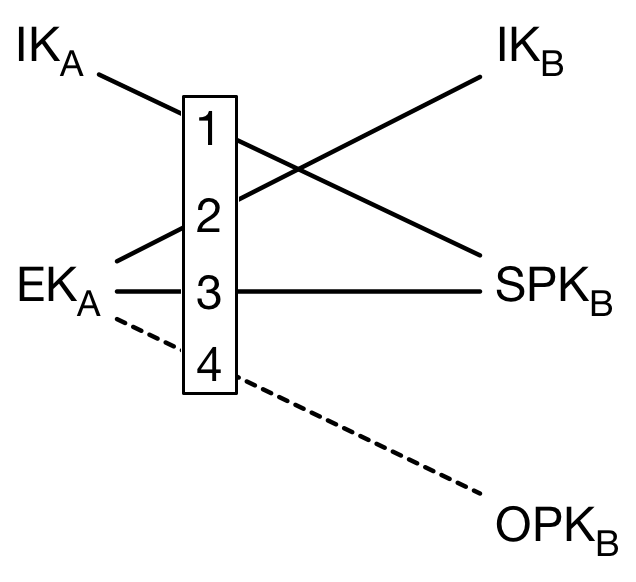
\includegraphics[width=0.3\textwidth]{image/X3DH}
    \caption{The procedure of computation}
    \label{x3dh1}
\end{figure}

In the pattern, $DH_1$ and $DH_2$ provide mutual authentication for Alice and Bob, $DH_3$ and $DH_4$ provide forward encryption. After the computation of SK, Alice delete the private key of the temporary key pair and the intermediate output value. Then Alice computes corresponding AD string the associated data containing the identification information of Alice and Bob:
$$AD=Encode(IK_A)||Encode(IK_B)$$


Alice can add additional information like the usernames, certificates and other marking information of Alice and Bob when computing $AD$.

After above key exchange procedure, Alice sends Bob an initial message including:
\begin{itemize}
    \item $IK_A$: Alice's identification key
    \item $EK_A$: Alice's temporary key
    \item the marking for choosing which $OPK_B$
    \item initial ciphertext encrypted by AEAD, which using $AD$ as associated data and one encryption key, which can be $SK$ or SK-encrypted PRF output.
\end{itemize}
Then Alice can use $SK$ and keys derived from $SK$ to communicate with Bob.

\paragraph{Bob receiving the initail message}
Bob retrieves the identification key $IK_A$ and temporary public key $EK_A$ of Alice from the initial message received from Alice and loads the relative private keys of his identification key $IK_B$, $SPK_B$ and $OPK_B$ used by Alice. Bob redo the DH and KDF computation mentioned above to generate $SK$ and delete the output value of DH. After these, Bob constructed AD string with $IK_A$ and $IK_B$. Finally, Bob tries to decrypt the initial ciphertext with $SK$ and $AD$. If the decryption fails, Bob will stop the protocol and delete $SK$ immediately, or else the protocol completes and Bob will delete the $OPK$ for forward encryption. Then Bob and use $SK$ or derived keys of $SK$ to perform the post-X3DH protocol with Alice.

\subsubsection{Double Ratchet}
The ratchet is a one-way gear. Through the ratchet algorithm, you can ensure that if someone gets the key, they can only decrypt the current data, but cannot monitor the previous or future data. The double ratchet is a forward one. The backward ratchet guarantees the security of forward and backward, and provides double insurance for the security of data transmission. Even the serial key can only read a small part of the data\cite{perrin2016double,cohn2016post}.

Signal Protocol uses a ratchet algorithm to generate a message key. Using a ratchet algorithm, each message can use a different key. Even if the key of a message is cracked, third parties can only calculate the key of the subsequent message, but not to the key to the previous message is called forward security.

If an additional ratchet algorithm is added, it can ensure backward security on the basis of forward security, that is, even if the key of a message is cracked, and the key of the message before and after cannot be cracked. This algorithm is called Double Ratchet algorithm. The Double Ratchet algorithm used by Signal Protocol in the communication between the two parties is KDF chain ratchet and DH ratchet to ensure the forward security and backward security of the message.

\paragraph{KDF chain}
KDF is a cryptographic function that inputs a secret and random KDF key and other data (see Figure \ref{kdfchain}), and returns the output data. Under the premise that the key is unknown, the output data is inseparable from the random number, which meets the PRF requirements in cryptography, that is, a pseudo-random function is reached. The KDF chain uses a part of KDF output as the output key, and another part as the next key\cite{bellare2017ratcheted}.

\begin{figure}[H]
    \centering
    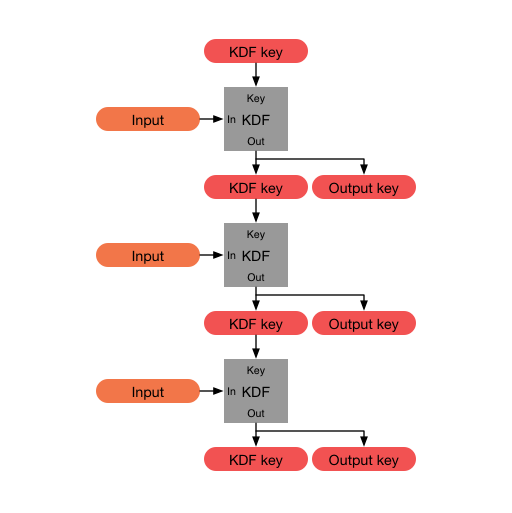
\includegraphics[width=0.6\textwidth]{image/KDFchain}
    \caption{KDF chain}
    \label{kdfchain}
\end{figure}

There are some features of KDF chain:
\begin{itemize}
    \item Resilience: For an attacker who does not know the KDF key, the output key looks random. Even if the attacker can control the input of KDF, this feature still holds.
    \item Forward security: For an attacker who knows the KDF key at a certain moment, the old output key looks random.
    \item Break-in recovery: For an attacker who knows the KDF key at a certain moment, the new output key looks random, as long as enough entropy is added to the new input.
\end{itemize}

This KDF chain is the root chain, sending chain, and receiving chain that need to run through the entire session.

When Alice and Bob exchange messages, they also exchange the new Diffie-Hellman public key, and the key output by Diffie-Hellman will be used as the input of the root chain. The key output by the root chain will be used as the KDF key of the sending chain and the receiving chain. This is called Diffie-Hellman ratchet.

Every time a message is sent and received, both the sending chain and the receiving chain will move forward. The corresponding output key will be used to encrypt and decrypt the message. This is called symmetric-key ratchet.

In this way, a double ratchet is formed, forming a forward and backward security guarantee.

\paragraph{Symmetric-key ratchet}

Each message sent or received is encrypted with a unique message key. The message key is the output key of the sending KDF chain and the receiving KDF chain. The KDF keys of these chains are called chain keys\cite{poettering2018towards}.

Since the KDF input of the sending chain and the receiving chain is constant, the two chains do not have the recoverability after being broken. The sending chain and receiving chain can only ensure that each message is encrypted with a unique key, and this key can be deleted after encryption or decryption. The process of calculating the next chain key and message key from a given chain key is called a ratchet step of a symmetric-key ratchet (Figure \ref{skratchet}).

\begin{figure}[H]
    \centering
    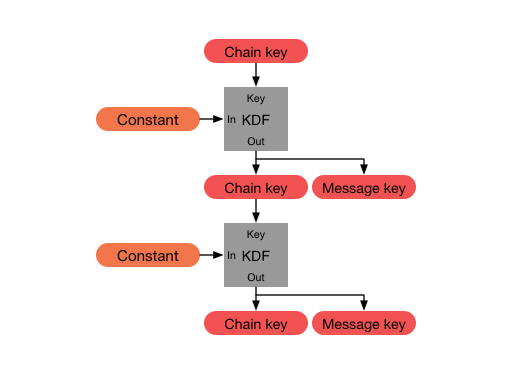
\includegraphics[width=0.6\textwidth]{image/skratchet}
    \caption{Symmetric-key ratchet}
    \label{skratchet}
\end{figure}



\paragraph{Diffie-Hellman Ratchet}
If the attacker steals one of the sending chain key and receiving chain key, then he can calculate all the message keys thereafter and decrypt the corresponding message. To avoid this, the double ratchet algorithm combines a symmetric key ratchet with a DH ratchet, and uses the latter to update the chain key based on the output of Diffie-Hellman\cite{almuzaini2019formal,cohn2018ends}.

In order to implement DH ratcheting, both parties to the communication generate a DH key pair (Diffie-Hellman public key and private key) as the current ratchet key pair. Each message sent from either party will carry a message header, which contains the sender's current ratchet public key. When receiving a new ratchet public key sent from the far end, the local end will implement a DH ratchet step (DH ratchet step) to generate a new ratchet key pair to replace the current local key pair.

Alice uses Bob's ratchet public key to initialize, and Bob has not yet learned of Alice's ratchet public key. As part of the initialization, Alice uses her own ratchet private key and Bob's ratchet public key for DH operations.

In this round, Alice also uses Bob's new public key to calculate a new round of DH steps.

Similarly, as the key calculated by DH changes, the sending chain will also step forward. Take the DH output as the KDF input of the root chain, and the KDF output of the root chain as the sending chain key and receiving chain key. So a complete DH ratchet step includes two updates of the root KDF chain, and its KDF output is used as the new receiving chain key and sending chain key.

\paragraph{Double Ratchet}
The combination of the symmetric key ratchet and the DH ratchet forms a double ratchet, which guarantees the security of forward and backward\cite{alwen2019double,cohn2017formal,poettering2018towards}.

When sending or receiving a message, a symmetric key ratcheting step of the sending chain or receiving chain is performed once to derive a new message key. When a new ratchet public key is received, before the symmetric key ratchet step, a DH ratchet step is performed to update the chain key\cite{perrin2016double}.

Alice has used Bob's ratchet public key and shared key initialization as the initial root key (RK). As part of the initialization, Alice generates a new ratchet key pair and uses the DH output as the input of the root KDF to calculate the new root key (RK) and send chain key (CK).

When Alice sends the first message A1, she performs a symmetric key ratchet step on the sending chain key to generate a new message key (the message key is marked with the message number it encrypted or decrypted). The new chain key will be saved, but the message key and the old chain key can be deleted.

Double ratchet stepping requires that both parties interact with each other to achieve a stepping. If the message is unilaterally sent or received, only symmetric key stepping occurs. DH stepping requires the other party to reply with a new ratchet public key.

When the new public key is received, the message key is calculated using the last time own private key, and the received message is decrypted. Then generate a new ratchet key pair for DH stepping, calculate a new message key, and encrypt the next message sent.




% \subsubsection{Curve25519}

% Curve25519 is currently the highest level of Diffie-Hellman function, suitable for a wide range of scenarios, designed by Professor Daniel J. Bernstein. In cryptography, Curve25519 is an elliptic curve that provides 128-bit security and is designed for elliptic curve Diffie-Hellman (ECDH) key agreement schemes. It is one of the fastest ECC curves and is not covered by any known patents.

% Given a user's 32-byte key, curve25519 calculates the user's 32-byte public key. Given this user's 32-byte key and another user's 32-byte public key, curve25519 calculates a 32-byte shared key and provides it to these two users. You can then use this secret to authenticate and encrypt two users.


\subsection{Issue1: Group chatting}
%TODO: Group chatting is one of the important functions in the online messaging application. Users within the group should be able to communicate with each other securely; A users should be allowed to join or leave the group; messaging server should not be able to know the sensitive information regarding the group member identities, message content and so on.You are required to define the security goals in detail that you believe to be reasonable in the group chatting scenario, and provide the solution based on the Signal framework. [2,3,4]

In secret conversation, each device should construct a pairwise channel with some other one device. The pairwise channel contains two devices: Initiator device and Responder device(denoted as I and R). The protocol use HKDF as a secure hash-based key derivation function and ECDH (Elliptic curve Diffie-Hellman) function applied to a secret and public key. Followed by the following steps, a new pairwise channel is generated following the X3DH protocol:
\begin{enumerate}
    \item Initiator obtains from server $IK_{pk}^R$, $SPK_{pk}^R$ and $OPK_{pk}^R$ for an one-time pre-key keypair genetated by the Responder device.
    \item Server then delete $OTPL^R_{pk}$ from the Responder's list of available one-time pre-keys, so long as it is not the last-resort.
    \item The Initiator generates a fresh ephemeral keypair $(EK^I_{sk},EK^I_{pk})$
    \item The Initiator then computes the first root key $RK$:
          $$a=ECDH(IK^I_{sk},SPK^R_{pk})$$
          $$b=ECDH(EK^I_{sk},IK^R_{pk})$$
          $$c=ECDH(EK^I_{sk},SPK^R_{pk})$$
          $$d=ECDH(EK^I_{sk},OTPK^R_{pk})$$
          $$RK=HKDF(a||b||c||d)$$
          Using the $RK$ the Initiator can calculate the first $CK$ and $MK$ and use those to start sending messages.
    \item The Initiator sends the first encrypted message to the Responder, including the fresh $EK_{pk}^I$ it generated previously.
\end{enumerate}

If the first encrypted message is received by Responder, then:
\begin{enumerate}
    \item Responder recomputes $RK$ through ECDH operations using the other part of the same keypairs available locally.
    \item Responder recomputes the first $CK$ and $MK$, and decrypts the message.
    \item Responder deletes $(OTPK_{pk}^R,OTPK_{sk}^R)$ from its local storage.

\end{enumerate}

For group chatting, more than 2 parties are involved in the protocol (Figure \ref{groupchatting}). The Signal Protocol’s Group Messaging protocol is used in secret conversations with more than two devices. All messages have a Sender and at least two Receivers. Prior to sending to a multi-device conversation Sender must have a pairwise channel with every Receiver. Sender also generates a $SCK$ (Sender Chain Keys, 256-bit values used to derive Sender Message Keys) and $SSK$ (Sender Signing Keys, key pairs used to sign multicast messages), and sends them along its pairwise channel to each Receiver.

Each multi-device message is encrypted with AES-CBC and signed by the $SSK$. The unique $SMK$ (Sender Message Keys, 384-bit values consisting of 256 bits for an AES-256 key, and 128 bits for an Initialization Vector ($IV$) for AES-CBC encryption.) is derived from the $SCK$ similarly to the pairwise channel:
$$SMK=HKDF(SCK)$$
For subsequent messages the Sender ratchets the $SCK$ using HKDF
$$SCK'=HKDF(SCK)$$
and uses each subsequent $SCK_0$ key to derive $SMK$ and $SSK$. This approach provides forward secrecy, as earlier $SCK$s and SMKs cannot be calculated from the current state. When a new device is added to a secret conversation, each other device will send the new device their latest $SCK$ upon sending their next message. When a device is removed however, each device will generate a new $SCK$. This ensures that the necessary key material is restricted to the devices within the thread.

If attachments like images, videos and voice records are considered, they should be encrypted and uploaded to server. The sender perform folloing operations:
\begin{enumerate}
    \item Sender generate a pseudo-random 256bit AES key $K$ and a 96-bit pseudo-random Initialization Vector $IV$.
    \item Sernder encrypts the attachment using AES-GCM encryption with K and IV. The header of the GCM encryption contains the $IV$.
    \item Sender computes a SHA256 hash H of the encrypted file and upload it to server. A unique identifier for tuture retireval can be obtained by the sender.
    \item Unique identifier, $K$, $H$ and attachment metadata are encoded into a message, which is encrypted and sent to the receivers having downloaded the content, who can verify the hash and decrypts the file with $K$.
\end{enumerate}

\begin{figure}[H]
    \centering
    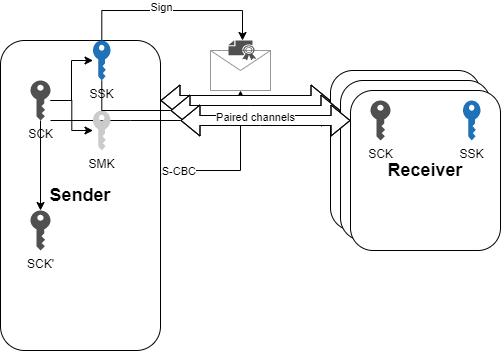
\includegraphics[width=0.6\textwidth]{image/groupchatting}
    \caption{The group chatting}
    \label{groupchatting}
\end{figure}



\subsubsection*{Security analysis}

The server only saves the client authentication public key (public authentication key), so even if being cracked, the attacker cannot decrypt the privacy content of users.

Considering authentication, no cryptographic guarantee of the authenticity of communicating parties is provided in the Signal Protocol. Public keys should be verified out-of-band using another communication channel. Without it, the communication could already be intercepted using a man-in-the-middle attack.

From the security perspective of Post-Quantum, all communication records may be preserved in cloud server.All data cannot be decrypted in the current situation, while may be decrypted in the case of quantum computer application. The quantum computers will be able to crack all asymmetric systems used in the Signal Protocol.

\subsection{Issue2: E2EE security except for Auditing}

%TODO: There are many popular messaging services which do not satisfy the E2EE security level, especially for the non-open source products. This is sometimes due to the auditing or other requirements by both the government and the company itself. Please provide the solution for this scenario so that the security requirements are satisfied as in the E2EE scenario except for the case that the messaging server is able to audit the corresponding communication session (message content, and user identity and so on). Please describe how you can limit the damage if the messaging server is compromised.

The surveillance of message is the rigid demand for public security and anti-terrorism. In the scenerio of E2EE, the bruceful cracking is impossible. However, E2EE does not avoid the security risks of the terminal itself. Each user's computer and other devices still have the possibility of encryption theft (for man-in-the-middle attacks), or the decrypted information is transformed. Even the most perfect encrypted communication, its security is still subject to the security of the sender and responder at both ends.

Based on this, MITM (Man-in-the-middle attack) method should be taken into concern. The legal institutions such as the server, the security departments or governments may perform some kind of "legitimate MITM" for any suspitious communication session. They do not need to fake identity as CA can provide legal digital certificates for the government, which prevent illegal eavesdroppers who are not legally authenticated and assigned legal digital certificates from performing MITM to common users.

In the surveillance concern, the monitor party, the sender Alice and receiver Bob actually form group chatting to a degree. Only those who has legal digital certificates from PKI (Public Key Infrastructure) can join the pairwise communication session. The security is proved in group chatting part. When an outsider tries to join the session, it should also perform X3DH with all the participants in the private session. The Identification Key $IK_{pk}^o$ should be associated with a certificate that can prove the identification of outsider. If the certificate fail to verify, which means it is untrusted attacker, the connection will be rejected, like Figure \ref{suv}.

\begin{figure}[H]
    \centering
    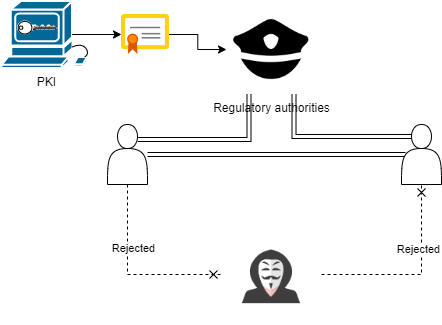
\includegraphics[width=0.6\textwidth]{image/suv}
    \caption{The surveillance of authorized departments}
    \label{suv}
\end{figure}


\section{Conclusion}
In this article, we presented the solutions to the issue of group chatting and messaging session auditing. As the Signal protocol realizes forward security and backward security for pairwise channel between sender and receiver through X3DH key exchange and Double Ratchet mechanism. The group messaging extended the participants by introducing more pairwise channels, where each multi-device message is encrypted. The forward security can be proved. For the surveillance concern, the messaging server may acquire digital certificate to perform legal auditing-term MITM in the private messaging session by extending it as group messaging, where server acts like transparent monitor.

\bibliography{wpref}

\end{document}
